\documentclass[oneside, a4paper, onecolumn, 11pt]{article}

% Change this: Customize the title, author, advisor, abstract
\newcommand{\thesistitle}[0]{Quantification of generalized measurement
incompatibility of mutually unbiased bases}
\newcommand{\authorname}[0]{Raul-Andrei Pop}

\newcommand{\supervisor}[0]{Marc-Olivier Renou and Lucas-Amadeus Tendick}
\newcommand{\supervisorinstitution}[0]{Inria Paris-Saclay / LIX}

\newcommand{\abstracttext}[0]{%

}

\usepackage[
  left=2cm,top=2.0cm,bottom=2.0cm,right=2cm,
  headheight=17pt, % as per the warning by fancyhdr
  includehead,includefoot,
  heightrounded, % to avoid spurious underfull messages
]{geometry}

\usepackage{dsfont}
\usepackage{optidef}
\usepackage{stmaryrd}
\usepackage[T1]{fontenc}
\usepackage{amstext}
\usepackage{amsmath}
\usepackage{amssymb}
\usepackage{amsthm}                          % definition / theorem environments
\usepackage{braket}    
\usepackage{bbm}                      % \ket{}, \bra{}, \braket{}{}

% Theorem-like environments (shared counter, numbered by section)
\theoremstyle{definition}
\newtheorem{definition}{Definition}[section]
\theoremstyle{plain}
\newtheorem{theorem}[definition]{Theorem}
\newtheorem{lemma}[definition]{Lemma}
\newtheorem{proposition}[definition]{Proposition}
\newtheorem{corollary}[definition]{Corollary}
\theoremstyle{remark}
\newtheorem*{remark}{Remark}
\usepackage{url}
\usepackage{graphicx}
\graphicspath{{./}{../assets/}}              % search current dir, then ../assets/
\usepackage{wrapfig}
\usepackage{placeins}                        % \FloatBarrier --- pin floats inside their section
\usepackage{enumerate}
\usepackage{paralist}
\usepackage{xspace}
\usepackage{color}
\usepackage{times}
\usepackage{listings}                        % source-code listings (appendix)

% --- Python listing style ---------------------------------------------------
\definecolor{codegreen}{rgb}{0,0.5,0}
\definecolor{codeblue}{rgb}{0,0,0.6}
\definecolor{codepurple}{rgb}{0.5,0,0.4}
\definecolor{codegray}{rgb}{0.5,0.5,0.5}
\lstdefinestyle{python}{
  language=Python,
  basicstyle=\ttfamily\footnotesize,
  keywordstyle=\bfseries\color{codeblue},
  commentstyle=\itshape\color{codegreen},
  stringstyle=\color{codepurple},
  showstringspaces=false,
  numbers=left,
  numberstyle=\tiny\color{codegray},
  numbersep=8pt,
  frame=single,
  framesep=4pt,
  breaklines=true,
  breakatwhitespace=true,
  columns=fullflexible,
  tabsize=2,
}
\usepackage[colorlinks,linkcolor=blue]{hyperref}
\usepackage[colorinlistoftodos,prependcaption,textsize=normal]{todonotes}
\usepackage{pdfpages}
\usepackage{fancyhdr} %% For changing headers and footers

\usepackage{titling}
\usepackage[nottoc,numbib]{tocbibind}

%% \predate{}
%% \postdate{}
%% \date{}
%% \author{\authorname}


\begin{document}

%\title{\thesistitle}

%\maketitle

% Max 10 lines.
%\noindent \paragraph*{Abstract}
%\abstract

\hspace{0pt}
\vfill

\begin{center}


\includegraphics[width=0.3\textwidth]{logo-EP-vertical}

\vspace*{2em}
%
{\large
\textbf{\'Ecole Polytechnique}

\vspace*{1em}
\textit{Lab Research Project Report}


\vspace*{3em}
{\Huge \textbf{\thesistitle}}
\vspace*{3em}



\textit{Author:}

\vspace*{1em}
\authorname{}, \'Ecole Polytechnique

\vspace*{2em}
%
{\textit{Advisor:}}

\vspace*{1em}
\supervisor{}
\\ \supervisorinstitution{}
}

\vspace*{2em}
\textit{Academic year 2025/2026}

\end{center}

\vfill
\hspace{0pt}

\newpage

\vfill
\noindent\textbf{Abstract}\\[1em]
%
\fbox{
\parbox{\textwidth}{
\abstracttext{In this work we will explore the problem 
of quantifying the incompatibility of mutually 
unbiased bases (MUBs) in finite-dimensional Hilbert spaces. We will reproduce 
the known results on the noise-robustness thresholds for the joint 
measurability of $k$ MUBs in prime dimensions, and we will present new 
numerical results obtained by solving semidefinite programs (SDPs) for generalized
incompatibility notions where closed-form expressions are not found yet. 
In producing these numerical results, we will provide a more general framework for quantifying these robustness thresholds by 
parameterizing the SDPs with arbitrary compatibility hypergraphs, which allows us to explore a wider range of compatibility scenarios beyond full joint measurability.
In an attempt to solve the problem analytically, we find analytical lower bounds for the noise-robustness thresholds on these incompatibility scenarios,
which match, up to machine precision, the numerical results.
%  We will also discuss the implications of our findings for quantum information processing tasks that rely on 
% MUBs, such as quantum state tomography and quantum cryptography. Finally, we 
% will outline some open questions and future directions for research in this area.
}
}
}
\vfill


\newpage

% Setting up the header
\pagestyle{fancy}
%\renewcommand{\headrulewidth}{0pt} % Remove line at top
%\renewcommand{\headrulewidth}{0.4pt}% Default \headrulewidth is 0.4pt
\lhead{\authorname}
%\chead{\acronym}
\rhead{\thesistitle}



\newpage
\tableofcontents
\newpage

%\pagenumbering{arabic}

%======================================================================
\section{Introduction}
 
Quantum theory and classical physics are fundamentally different even at the level of
measurement: quantum measurements are probabilistic and measuring them disturbs, hence, changes the state. Therefore, not every collection of observables can be read out at the same
time. Classically, any set of physical quantities can in principle be measured
jointly to arbitrary precision, so that a single experiment reveals the value
of all of them. In quantum mechanics this is no longer true. There exist sets
of measurements that are \emph{incompatible}, in the sense that no single
apparatus supplemented only by classical processing of its outcomes can
reproduce their statistics. Historically, this feature was first recognised
through the non-commutativity of observables, $AB \neq BA$, and the uncertainty
relations it entails. From a modern, information-theoretic standpoint, however,
incompatibility is much more than a curiosity: it is a necessary ingredient of
essentially every genuinely non-classical effect. The violation of Bell
inequalities, Einstein--Podolsky--Rosen (EPR) steering, and quantum
contextuality all require incompatible measurements, and incompatibility acts
as a resource in tasks such as quantum key distribution, quantum state
discrimination, and quantum random access codes~\cite{Quintino2019,Guhne2023}.
 
The operationally meaningful way to formalise this notion is
\emph{joint measurability}. The commutator, while adequate for projective
measurements, is too narrow to characterise the most general measurements
allowed by quantum mechanics, the positive operator-valued measures (POVMs).
Instead, a family of POVMs is said to be jointly measurable, or
\emph{compatible}, if there is a single \emph{parent} POVM whose outcomes can be
classically post-processed to recover each measurement of the family; if no such
parent exists the measurements are \emph{incompatible}
(see Definition~\ref{def:jm}). This definition reduces to
commutativity for projective measurements but is strictly more permissive in
general: there are non-commuting POVMs that nonetheless admit a joint
measurement~\cite{Guhne2023}.
 
Among all quantum measurements, those associated with \emph{mutually unbiased
bases} (MUBs) are the prototypical candidates for being ``maximally
incompatible.'' Two orthonormal bases of a $d$-dimensional Hilbert space are
mutually unbiased when the overlap of any vector of one basis with any vector of
the other has constant modulus, $|\langle b_i | b_j' \rangle|^2 = 1/d$, so that
preparing the system in an eigenstate of one basis renders the outcome of a
measurement in the other completely random. The eigenbases of the three Pauli
operators provide the canonical example in dimension two, and MUBs are commonly
regarded as the higher-dimensional generalisation of the Pauli
measurements~\cite{Designolle2019}.
 
To turn the binary question ``compatible or not'' into a quantitative one, one
mixes each measurement with white noise. Writing $\Pi^{(j)}_a$ for the projector
onto the $a$-th vector of the $j$-th basis, the $\eta$-noisy MUB measurement has
elements
\begin{equation}
  M^{\eta}_{a|j} \;=\; \eta\,\Pi^{(j)}_a \;+\; (1-\eta)\,\frac{I}{d},
  \qquad j \in \llbracket 1, k \rrbracket,\; a \in \llbracket 1, d \rrbracket,
\end{equation}
which is the general POVM white-noise mixture
$\eta\,M_a + (1-\eta)\,\mathrm{Tr}(M_a)\,I/d$ of \eqref{eq:noisy-povm}
specialised to rank-1 projectors -- here $\mathrm{Tr}(\Pi^{(j)}_a) = 1$,
so the trace factor collapses to unity. One then asks for the largest
noise parameter $\eta^\star$ below which the family becomes jointly
measurable. This \emph{white-noise robustness} is the figure of
merit used throughout this report; crucially, it can be computed by semidefinite
programming (SDP)~\cite{Designolle2019,Guhne2023}. For the full joint
measurability of $k$ MUBs in prime-power dimension $d$, Designolle, Skrzypczyk,
Fröwis and Brunner~\cite{Designolle2019} derived general upper and lower bounds
on $\eta^\star(k,d)$ that coincide in several important cases, in particular for
two MUBs in any dimension and for the complete set of $k = d+1$ MUBs.
 
The all-or-nothing notion of full joint measurability is, however, only the
coarsest description of how a set of measurements can be (in)compatible. Once
three or more measurements are considered, richer \emph{structures} of
compatibility appear: a triple can be pairwise compatible yet fail to be jointly
measurable as a whole, and one may distinguish, for instance, genuine $k$-wise
incompatibility from weaker forms. Quintino \emph{et al.}~\cite{Quintino2019}
organised these possibilities through \emph{compatibility hypergraphs}, in which
each hyperedge collects a subset of measurements required to be jointly
measurable, and showed how the corresponding robustness can again be cast as an
SDP. While the noise robustness of full joint measurability of MUBs is by now
well charted, these intermediate scenarios remain largely unexplored
quantitatively.
 
This report addresses precisely that gap. Our contributions are fourfold.
First, we reproduce the known noise-robustness thresholds for the joint
measurability of $k$ MUBs by explicitly formulating and solving the
corresponding SDPs, recovering the closed-form values
of~\cite{Designolle2019}. Second, we provide a general framework in which the
robustness SDP is parameterised by an \emph{arbitrary} compatibility hypergraph,
allowing us to interpolate between full joint measurability and weaker
compatibility scenarios such as the convex combination of pairwise compatibility of $k$ MUBs.
Third, we report new numerical values for these generalised incompatibility
notions, for which no closed-form expression is yet known. Finally, we derive
analytical lower bounds for the corresponding thresholds and show that they
match our numerical results up to machine precision, which suggests that the
underlying optimal strategy is an equal-probability mixture of all pairwise
sub-experiments.
 
%======================================================================
%  Section 2 --- Background
%======================================================================
\section{Background}
 
\paragraph{Non-commutativity and the rise of joint measurability.}
The peculiar status of measurement in quantum theory was apparent from the very
beginning. In 1925 Heisenberg observed that the product of physical quantities
may depend on their order, a remark that Born and Jordan immediately traced back
to the matrix nature of observables, $AB \neq BA$~\cite{Guhne2023}. The ensuing
uncertainty relations, of Heisenberg, Kennard and Robertson, tied
non-commutativity to the impossibility of preparing states sharply localised
with respect to two observables at once. It was later realised that the notion of observables associated to projective measurements
is too restrictive to capture all physical measurements, and the
notion of a measurement was generalised to POVMs. For this larger class the
commutator no longer tells the whole story, and over the past two decades joint
measurability has emerged as the central, operationally grounded notion of
compatibility, with deep links to Bell nonlocality, EPR steering, contextuality
and a range of information-processing tasks~\cite{Quintino2019,Guhne2023}.
 
\paragraph{Mutually unbiased bases.}
Schwinger introduced what we now call mutually unbiased bases in his 1960
\emph{PNAS} paper on unitary operator bases, as a tool for representing pairs of
``maximally non-commuting'' measurements~\cite{Schwinger1960}. Wootters and
Fields~\cite{WoottersFields1989} established that at most $d+1$ MUBs can exist in
dimension $d$, and gave an explicit construction of complete sets of $d+1$ MUBs
whenever $d = p^{r}$ is a power of a prime. Whether this bound can be saturated
in composite (non-prime-power) dimensions is a long-standing open problem; the
smallest open case is $d = 6$, where despite considerable effort no more than
three MUBs have ever been found and it is widely conjectured that no fourth one
exists. In this report we work exclusively in prime dimensions $d \in
\{2,3,5,7, 11\}$, where the Wootters--Fields construction provides explicit complete
sets to build on. Beyond their role as extremal incompatible measurements, MUBs
are ubiquitous in quantum information processing, appearing in quantum
tomography, uncertainty relations, quantum key distribution and entanglement
detection~\cite{Designolle2019}.
 
\paragraph{Joint measurability as a semidefinite program.}
The question of whether a set of POVMs is jointly measurable can be decided by
convex optimisation. A key simplification is that the classical post-processing
in the definition of joint measurability may, without loss of generality, be
taken to be deterministic, so that only finitely many response functions need to
be considered~\cite{Guhne2023}. For two binary qubit POVMs, Wolf, P\'erez-Garc\'ia
and Fern\'andez recast compatibility as the existence of a single
positive-semidefinite operator satisfying linear constraints, which is a small
feasibility SDP. For a general family $\{M_{a|x}\}$, deciding compatibility
amounts to searching for a parent POVM $\{G_\lambda\}$ whose deterministic
marginals reproduce every $M_{a|x}$, and this too is an SDP. Replacing the
feasibility question by a maximisation over the noise parameter $\eta$ turns the
program into one whose optimal value is exactly the white-noise robustness.
Modern interior-point solvers (e.g.\ \textsc{Clarabel}, \textsc{SCS},
\textsc{Mosek}) handle these programs routinely.
 
\paragraph{Quantifying incompatibility: noise robustness.}
Just as in entanglement theory one quantifies how far a state is from being
separable by adding noise, one quantifies how far a set of measurements is from
being compatible. Mixing each POVM with a fraction of white noise as
in~Eq.~(1) and asking for the critical $\eta^\star$ defines the
\emph{(white-)noise robustness}, an incompatibility monotone introduced in this
context by Heinosaari, Kiukas and Reitzner and studied as an SDP by Cavalcanti
and Skrzypczyk and others~\cite{Heinosaari2015,Designolle2019,Guhne2023}.
Related quantifiers, such as the incompatibility weight and the (generalised)
incompatibility robustness, arise by allowing other noise models, and all share
the property of being non-increasing under suitable free operations. For MUBs
specifically, Designolle \emph{et al.}~\cite{Designolle2019} obtained, via the
dual SDP, a general upper bound on $\eta^\star$ and an analytical lower bound
that uses only the unbiasedness relation. These bounds are tight in several
families; in particular,
\begin{equation}
  \eta^\star(2,d) \;=\; \frac{2+\sqrt{d}}{2(\sqrt{d}+1)},
  \qquad
  \eta^\star(d+1,d) \;=\; \frac{1}{\sqrt{d+1}},
\end{equation}
the former giving $\eta^\star(2,2) = 1/\sqrt{2}$ for the two Pauli MUBs of a
qubit. These closed forms populate the reference table of thresholds that we
reproduce in Section~\ref{sec:results}.
 
\paragraph{Structures of incompatibility.}
For sets of three or more measurements, compatibility is no longer a single
yes/no property but a structured one. Heinosaari, Reitzner and Stano exhibited
triples of qubit measurements that are pairwise jointly measurable but not
jointly measurable as a whole, and Kunjwal, Heunen and Fritz showed that, for
large enough sets, essentially arbitrary joint-measurability structures can be
realised in quantum mechanics~\cite{Guhne2023}. Quintino
\emph{et al.}~\cite{Quintino2019} formalised this through compatibility
hypergraphs $\mathcal{C} = [C_1,\dots,C_N]$, where each hyperedge $C_i$ lists a
subset of measurements that must be compatible, and through
the notion of \emph{genuine $\mathcal{C}$-incompatibility}: a family is
genuinely $\mathcal{C}$-incompatible if it cannot be written as a convex
combination of families respecting the structures $C_i$.

\begin{figure}[h]
  \centering
  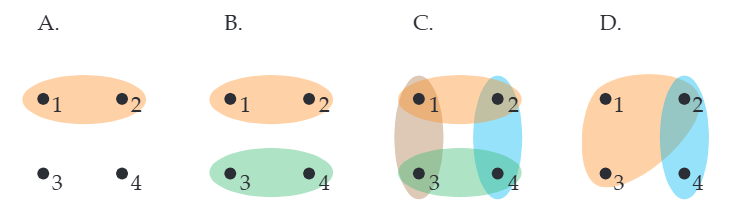
\includegraphics[width=0.85\textwidth]{hypergraphs.png}
  \caption{Examples of compatibility hypergraphs on $n = 4$ measurements,
           reproduced from Fig.~1 of Quintino \emph{et al.}~\cite{Quintino2019}.
           Each node represents a complete measurement (a POVM); each
           hyperedge, drawn as a coloured region, groups measurements that
           are required to be jointly measurable. Vertices not contained in
           any hyperedge are incompatible with the rest. From left to right:
           $\mathcal{C}_A = [(1,2)]$,
           $\mathcal{C}_B = [(1,2),(3,4)]$,
           $\mathcal{C}_C = [(1,2),(1,3),(2,4),(3,4)]$,
           $\mathcal{C}_D = [(1,2,3),(2,4)]$. The all-pair hypergraph studied in depth in this work corresponds to C.}
  \label{fig:hypergraphs}
\end{figure} The canonical instance is genuine
$n$-wise incompatibility, in which a set of $n$ measurements cannot be
decomposed into a mixture of $(n-1)$-wise compatible ones. As in the case of
ordinary joint measurability, deciding genuine $\mathcal{C}$-incompatibility and
quantifying its noise robustness can be phrased as semidefinite
programs~\cite{Quintino2019}. It is exactly this hypergraph-parameterised
viewpoint that we adopt and implement in Section~\ref{sec:sdp}, in order to
quantify incompatibility scenarios for MUBs that lie between full joint
measurability and full independence.
 
%======================================================================

\section{Outline and goal of the project}

The goal of this project is to study, both numerically and analytically, the noise-robustness thresholds that quantify how incompatible mutually unbiased bases (MUBs) are as quantum measurements. Incompatibility is treated here not as a binary property but as a quantitative one: by mixing each MUB measurement with white noise at level $\eta \in [0,1]$ and asking for the largest $\eta$ below which the noisy family admits a given compatibility structure, we obtain a sharp figure of merit $\eta^\star$ that can in principle be computed by semidefinite programming. Within this framework, our objectives are the following.

\paragraph{Reproducing the joint-measurability baseline.} We first reproduce the known noise-robustness thresholds $\eta^\star(k,d)$ for the full joint measurability of $k$ MUBs in prime dimension $d$, derived in closed form by Designolle et al.~\cite{Designolle2019} for the special cases $k=2$ and $k=d+1$. Concretely, we formulate the corresponding SDP from scratch, implement it in CVXPY, and verify that the solver recovers the analytical values to within $10^{-4}$ across the full range of $(k,d)$ that is computationally tractable. This step both validates our implementation and produces the reference table against which the generalised scenarios are compared.

\paragraph{Generalising to arbitrary compatibility hypergraphs.} Following the hypergraph formalism of Quintino et al.~\cite{Quintino2019}, we then design and implement a single SDP whose constraints are parameterised by an arbitrary compatibility hypergraph $\mathcal{C}$. Each hyperedge of $\mathcal{C}$ specifies a subset of measurements that must admit a common parent POVM, while the remaining measurements in each branch are left as independent POVMs; the SDP searches for the largest $\eta$ such that the noisy MUB family decomposes as a convex mixture of such branches. The trivial hypergraph $\mathcal{C} = \{(0,1,\dots,k-1)\}$ recovers full joint measurability as a special case, so the standard problem becomes the simplest instance of a much broader family of compatibility scenarios that our code handles uniformly.

\paragraph{Producing new numerical thresholds for the all-pairs hypergraph.} Using this general framework, we compute new noise-robustness thresholds for the all-pairs compatibility hypergraph, in which the $k$ measurements are required to be only pairwise---rather than fully---jointly measurable, in a convex-mixture sense. Because this SDP scales only as $O(k^3 d^2)$ in the number of matrix variables, rather than as $O(d^k)$ for the full-JM SDP, we are able to populate a substantially larger range of $(k,d)$ values than is feasible for the joint-measurability case, up to $k=9$ in dimension $d=11$.

\paragraph{Deriving and certifying an analytical lower bound.} Finally, we exploit the symmetry of the MUB family to construct an explicit feasible point of the all-pairs SDP, given by the equal-weight mixture of all $\binom{k}{2}$ pairwise strategies. Combining this construction with the affineness of the white-noise map and the closed-form pairwise threshold $\eta^\star(2,d)$ from~\cite{Designolle2019}, we obtain the analytical lower bound
\begin{equation}
    \eta^\star_{\mathrm{pair}}(k,d) \;\geq\; 1 - \frac{\sqrt{d}}{k(\sqrt{d}+1)}.
\end{equation}
This bound is monotonically increasing in $k$, in sharp contrast to the full-JM threshold which decreases in $k$, and it matches our numerical SDP values to solver precision in every case we tested. The agreement strongly suggests that the equal-weight pairwise mixture is in fact optimal for this hypergraph, and that the bound is tight.

% \newpage
\section{Definitions and Concepts}

\subsection{Hermitian operators}

The definitions in this subsection are standard and follow the
presentation of \cite{Quantum-Computation-and-Quantum-Information}; we include them here for
self-containedness and to fix the notation used in the rest of the
report.

\begin{definition}[Pre-Hilbert space]
  A pair ($\mathcal{H}$, ⟨ , ⟩) composed of complex vector space E and an inner product ⟨ , ⟩ on E
is called a complex inner product space, or a complex pre-Hilbert space.
\end{definition}

\begin{definition}[Hermitian space]
  A finite-dimensional pre-Hilbert space is called a Hermitian space.
\end{definition}

\begin{definition}[Cauchy sequence]
  A sequence $(\psi_n)_{n \in \mathbb{N}}$ in a pre-Hilbert space $\mathcal{H}$ is called a Cauchy sequence if for every $\epsilon > 0$, there exists an $N \in \mathbb{N}$ such that for all $m, n > N$, we have $\|\psi_n - \psi_m\| < \epsilon$.
\end{definition}

\begin{definition}[Complete space]
  A pre-Hilbert space is called complete if every Cauchy sequence converges.
\end{definition}

\begin{definition}[Hilbert space]
  A complete pre-Hilbert space is called a Hilbert space.
\end{definition}

\begin{definition}[Adjoint of an operator in a Hilbert space]
  Let $\mathcal{H}$ be a complex Hilbert space. For any linear operator $A : \mathcal{H} \to \mathcal{H}$, there exists a unique linear operator $A^{\dagger} : \mathcal{H} \to \mathcal{H}$ such that
  \begin{equation}
    \langle \phi | A\psi \rangle = \langle A^{\dagger}\phi | \psi \rangle
  \end{equation}
  for all $\phi, \psi \in \mathcal{H}$. The operator $A^{\dagger}$ is called the adjoint of $A$.
\end{definition}

\begin{definition}[Hermitian operator]
\label{def:hermitian}
Let $\mathcal{H}$ be a complex Hilbert space. A linear operator
$A : \mathcal{H} \to \mathcal{H}$ is called \emph{Hermitian} (or
\emph{self-adjoint}) if it equals its own adjoint,
\begin{equation}
  A \;=\; A^{\dagger},
  \label{eq:hermitian}
\end{equation}
or, equivalently,
$\langle \phi | A\psi \rangle = \langle A\phi | \psi \rangle$
for all $\phi, \psi \in \mathcal{H}$.
\end{definition}
In finite dimension $\mathcal{H} = \mathbb{C}^{d}$, this reduces to the matrix
condition $A_{ij} = \overline{A_{ji}}$. Hermitian operators have real
eigenvalues and an orthonormal eigenbasis, which is why they model
physical observables in quantum mechanics.
\\ Also note that a Hermitian space (finite-dimenional pre-Hilbert space) is always complete, and thus it is a Hilbert space.
In this study we are only concerned with finite-dimensional Hilbert spaces. While we will use the term "Hilbert space", it is important to remember that 
the spaces we are working with are also Hermitian spaces.

\begin{definition}[Positive semidefinite operator]
  Let $\mathcal{H}$ be a complex Hilbert space. A linear operator $A : \mathcal{H} \to \mathcal{H}$ is called positive semidefinite if for all $\psi \in \mathcal{H}$, we have $\langle \psi | A\psi \rangle \geq 0$.
\end{definition}


\subsection{Quantum states, density operators and quantum measurements}
A quantum state is a mathematical object that fully describes the quantum
mechanical state of a physical system. It can be represented by a state vector in a complex Hilbert space or by
a density operator.
\begin{definition}[Quantum Bit (Qubit)]
  A qubit is a linear combination of the (orthonormal) computational basis states $\ket{0}$ and $\ket{1}$ in a two-dimensional complex Hilbert space $\mathcal{H} = \mathbb{C}^2$. A general state of a qubit can be written as
  \begin{equation}
    \ket{\psi} = \alpha \ket{0} + \beta \ket{1},
  \end{equation}
  where $\alpha, \beta \in \mathbb{C}$ and $|\alpha|^2 + |\beta|^2 = 1$.
  Upon measuring the qubit in the computational basis, the outcome will be $\ket{0}$ with probability $|\alpha|^2$ and $\ket{1}$ with probability $|\beta|^2$.


\end{definition}

\begin{definition}[Quantum state]
A quantum state can be described by a state vector $\ket{\psi}$ in a complex Hilbert space $\mathcal{H}$, where $\ket{\psi}$ is a unit vector (i.e., $\langle \psi | \psi \rangle = 1$). The state vector represents the pure state of a quantum system.  
\end{definition}

\begin{definition}[Pure state]
  A pure state is a quantum state that can be represented by a state vector $\ket{\psi}$ in a complex Hilbert space. It is called pure because it cannot be expressed as a convex combination of other states. A pure state corresponds to a rank-1 projector in the density operator formalism, i.e., $\rho = \ket{\psi}\bra{\psi}$.
\end{definition}

% \begin{definition}[Density operator]
% A density operator (or density matrix) $\rho$ is a positive semidefinite operator on
% a complex Hilbert space $\mathcal{H}$ with trace equal to 1, i.e., $\rho \geq 0$ and $\text{Tr}(\rho) = 1$. Density operators can represent both pure states (when $\rho$ is a rank-1 projector) and mixed states (when $\rho$ is a convex combination of pure states).
% \end{definition}
\begin{definition}[Density operator]
  A density operator (or density matrix) $\rho$ is a positive semidefinite operator on a complex Hilbert space $\mathcal{H}$ with trace equal to 1, i.e., $\rho \geq 0$ and $\text{Tr}(\rho) = 1$. Density operators can represent both pure states (when $\rho$ is a rank-1 projector) and mixed states (when $\rho$ is a convex combination of pure states).
  For a quantum state described by the set $\{p_i, \ket{\psi_i}\}$, where $p_i$ are probabilities and $\ket{\psi_i}$ are pure states, the corresponding density operator is given by
  \begin{equation}
    \rho = \sum_i p_i \ket{\psi_i}\bra{\psi_i}.
  \end{equation} 
\end{definition}

\subsection{Mutually unbiased basis (MUBs)}

\begin{definition}[Basis]
  Let $\mathcal{H}$ be a finite-dimensional complex Hilbert space, with $dim(\mathcal{H}) = d$. A set of vectors $\mathcal{B} = \{\ket{b_i}\}_{i \in I}$ is called a basis of $\mathcal{H}$ if every vector $\ket{\psi} \in \mathcal{H}$ can be uniquely expressed as a linear combination of the vectors in $\mathcal{B}$, i.e., there exist unique coefficients $c_i \in \mathbb{C}$ such that
  \begin{equation}
    \ket{\psi} = \sum_{i \in I} c_i \ket{b_i}.
  \end{equation}
\end{definition}

\begin{definition}[Orthonormal basis]
  A basis $\mathcal{B} = \{\ket{b_i}\}_{i=1}^d$ of a complex Hilbert space $\mathcal{H}$ is called orthonormal if for all $i, j \in \{1, \ldots, d\}$, we have
  \begin{equation}
    \langle b_i | b_j \rangle = \delta_{ij},
  \end{equation}
  where $\delta_{ij}$ is the Kronecker delta function, which equals 1 if $i = j$ and 0 otherwise.
  
\end{definition}

\begin{definition}[Mutually unbiased bases (MUBs)]
  Let $\mathcal{H}$ be a complex Hilbert space of dimension $d$. Two orthonormal bases $\mathcal{B} = \{\ket{b_i}\}_{i=1}^d$ and $\mathcal{B}' = \{\ket{b'_j}\}_{j=1}^d$ of $\mathcal{H}$ are called mutually unbiased if for all $i, j \in \{1, \ldots, d\}$, we have
  \begin{equation}
    |\langle b_i | b'_j \rangle|^2 = \frac{1}{d}.
  \end{equation}
  A set of orthonormal bases $\{\mathcal{B}_1, \ldots, \mathcal{B}_k\}$ is called mutually unbiased if every pair of distinct bases in the set is mutually unbiased.
\end{definition}

\subsection{Quantum Measurements}
\label{sec:quantum-measurements}

A quantum measurement is the formal device by which one extracts
classical information from a quantum state. Each measurement is
specified by a finite set of \emph{outcomes}
$\{a\}_{a = 1}^{n}$ together with an operator on the Hilbert
space~$\mathcal{H}$ for each outcome; the probability of each outcome
is then read off from the state via the Born rule below. We
distinguish two levels of generality, projective measurements and the
strictly larger class of POVMs.

\begin{definition}[Projective measurement (PVM)]
\label{def:pvm}
A \emph{projective measurement} on a complex Hilbert space $\mathcal{H}$
of dimension $d$ is a finite family $\{\Pi_a\}_{a = 1}^{n}$ of
orthogonal projectors on $\mathcal{H}$,
\begin{equation}
  \Pi_a^{\dagger} \;=\; \Pi_a, \qquad
  \Pi_a \Pi_b \;=\; \delta_{ab}\, \Pi_a, \qquad
  \sum_{a = 1}^{n} \Pi_a \;=\; I.
  \label{eq:pvm}
\end{equation}
By the spectral theorem, projective measurements are in one-to-one
correspondence with self-adjoint observables
$A = \sum_a \lambda_a\, \Pi_a$ on~$\mathcal{H}$, the $\lambda_a$
being the eigenvalues attached to each outcome.
\end{definition}

\begin{definition}[Positive operator-valued measure (POVM)]
\label{def:povm}
A \emph{positive operator-valued measure} (POVM) on a complex Hilbert
space $\mathcal{H}$ with outcome set $\{1, \dots, n\}$ is a family
$\{M_a\}_{a = 1}^{n}$ of Hermitian operators satisfying
\begin{equation}
  M_a \;\geq\; 0 \quad \forall\, a, \qquad
  \sum_{a = 1}^{n} M_a \;=\; I.
  \label{eq:povm-defining}
\end{equation}
Every projective measurement is a POVM (the $\Pi_a$ are positive,
Hermitian, and sum to the identity), but the converse fails: a POVM
element $M_a$ may have rank greater than one and the $M_a$ need not
mutually commute. POVMs are the most general notion of measurement
allowed by quantum mechanics; by Naimark's theorem every POVM arises
as a projective measurement on an enlarged Hilbert space, with the
extra degrees of freedom subsequently traced out.
\end{definition}

\begin{definition}[Born rule]
\label{def:born}
If the system is prepared in a state described by the density operator
$\rho$ and a POVM $\{M_a\}$ is performed, the probability of
observing outcome~$a$ is
\begin{equation}
  P(a \mid \rho) \;=\; \text{Tr}(\rho\, M_a).
  \label{eq:born}
\end{equation}
Positivity $M_a \geq 0$ together with the resolution of the
identity $\sum_a M_a = I$ guarantees that
$\{P(a \mid \rho)\}_{a = 1}^{n}$ is a valid probability distribution
on the outcome set for every density operator~$\rho$.
\end{definition}

\paragraph{Indexed families of POVMs.}
In what follows we shall study not a single POVM but \emph{collections}
of POVMs sharing the same Hilbert space and outcome set, indexed by a
classical measurement \emph{setting}~$x \in \{1, \dots, m\}$. We
adopt the standard notation $M^{(x)} = \{M_{a|x}\}_{a = 1}^{n}$ for
the POVM associated with setting~$x$, so that each $M_{a|x}$ is a
Hermitian operator on $\mathcal{H}$ satisfying
\eqref{eq:povm-defining} for every fixed~$x$, and the Born rule
extends naturally to $P(a \mid x, \rho) = \text{Tr}(\rho\, M_{a|x})$.
The central question of this report---developed in the next
subsection and formalised as a semidefinite program in
Section~\ref{sec:sdp-2qubit}---is to what extent such a collection
$\{M^{(x)}\}_{x}$ can be realised \emph{simultaneously} by a single
physical measurement.

\begin{definition}[White-noise mixture of a POVM]
\label{def:white-noise}
Given a POVM $\{M_a\}$ on $\mathcal{H} = \mathbb{C}^{d}$ and a noise
parameter $\eta \in [0, 1]$, the corresponding \emph{$\eta$-noisy}
POVM has elements
\begin{equation}
  M^{\eta}_{a} \;=\; \eta\, M_{a} \;+\; (1 - \eta)\, \text{Tr}(M_a)\,
                     \frac{I}{d}.
  \label{eq:noisy-povm}
\end{equation}
At $\eta = 1$ the original sharp measurement is recovered; at
$\eta = 0$ every outcome operator becomes proportional to the
maximally mixed state $I/d$, so the outcome distribution
$P(a \mid \rho)$ no longer depends on $\rho$ and the measurement is
uninformative. The parameter $\eta$ will serve as the quantitative
figure of merit of measurement incompatibility throughout the rest of
the report.
\end{definition}

\begin{lemma}[Affineness]
The map $\eta \mapsto M^\eta = \eta M + (1-\eta)\,\mathrm{Tr}(M)\,\frac{I}{d}$ is affine, so for any probabilities $\{q_b\}$ and noise levels $\{\eta_b\}$,
\[
\sum_b q_b\, M^{\eta_b} \;=\; M^{\,\sum_b q_b \eta_b}.
\]
\end{lemma}

%------------------------------
% TODO: born rule, Tr[...]    |
% complete section            |
%------------------------------

\subsection{Joint Measurability and Incompatibility}

\begin{definition}[Joint measurability] \label{def:jm}
  A set of quantum measurements (POVMs) $\{ M_{a|x} \}$ is said to be jointly measurable if there exists a single measurement (POVM) $\{G_\lambda\}$ such that the outcomes of $G$ can be post-processed to reproduce the statistics of each $M_{a|x}$.
  That is, there exists a set of conditional probabilities $p(a|x, \lambda)$ such that for all $x$ and $a$, we have
  \begin{equation}
    M_{a|x} = \sum_{\lambda} p(a|x, \lambda) G_{\lambda},
  \end{equation}
  In this case the POVM $\{G_\lambda\}$ is called a joint or parent
  measurement of the set $\{M_{a|x}\}$.
\end{definition}

A set of quantum measurements is \textbf{incompatible} if it is not jointly measurable.

\subsection{Semi Definite Programming (SDP)}
The feasibility and noise-robustness of measurement compatibility can be modeled as an SDP and computationally solved by convex optimization libraries, for example in Python or MatLAB.
For this reason, we will briefly review the definition of an SDP and some prerequisite concepts, and in the next section we will model our systems as SDPs.

\begin{definition}[Positive semidefiniteness of a Hermitian operator]
  A Hermitian operator $A$ is said to be positive semidefinite if for all vectors $\ket{\psi}$ in the Hilbert space, we have
  \begin{equation}
    \langle \psi | A | \psi \rangle \geq 0.
  \end{equation}
  We will denote this by $A \geq 0$.
\end{definition}

Note that we can further extend this (non-total) ordering of Hermitian operators like so
\begin{equation}
  A \geq B \quad \text{if and only if} \quad A - B \geq 0.
\end{equation}

\begin{definition}[Semidefinite Program]
  A semidefinite program is an optimization problem of the form
  \begin{equation}
    \begin{aligned}
      \text{minimize} \;\;& \text{Tr}(C X) \\[2pt]
      \text{subject to} \;\;& \text{Tr}(A_i X) = b_i, \quad i = 1, \ldots, m, \\[2pt]
                          & X \geq 0,
    \end{aligned}
  \end{equation}
  where $X$ is the variable being optimized over, $C$ and $A_i$ are given Hermitian matrices, and $b_i$ are given scalars.
  
\end{definition}

\newpage
\section{Joint Measurability SDP}\label{sec:sdp}
In this section, we will explore convex optimization programs for identifying jointly measurable sets of quantum measurements and quantifying their incompatibility by solving these programs for minimum noise on noisy measurements.
We aim to derive and implement a generalization of this program in order to obtain more numerical results on the genuine $k$-wise incompatibility problem introduced by Quintino et al.~\cite{Quintino2019}.

\subsection{A first example: two noisy Pauli measurements on a qubit}
\label{sec:sdp-2qubit}

To make the framework concrete, we begin with the smallest non-trivial
case: two binary-outcome POVMs on a single qubit, i.e.\ $d = 2$, $m = 2$
settings, $n_a = 2$ outcomes per setting. Take the eigenprojectors of
the Pauli observables $\sigma_X$ and $\sigma_Z$,
\begin{equation}
  \Pi^{(X)}_{\pm} \;=\; \frac{I \pm \sigma_X}{2},
  \qquad
  \Pi^{(Z)}_{\pm} \;=\; \frac{I \pm \sigma_Z}{2},
\end{equation}
and mix them with white noise at level $\eta \in [0,1]$,
\begin{equation}
  M^{\eta}_{a|x} \;=\; \eta\, \Pi^{(x)}_{a}
                  \;+\; (1-\eta)\, \frac{I}{2},
  \qquad x \in \{X, Z\},\;\; a \in \{+,-\}.
  \label{eq:noisy-pauli-2}
\end{equation}
By construction each $M^{\eta}_{a|x}$ is positive semidefinite and
$\sum_a M^{\eta}_{a|x} = I$, so $\{M^{\eta}_{\cdot\,|x}\}$ is a POVM for
every setting $x$ and every $\eta \in [0,1]$.

By the definition of joint measurability given above, the family
$\{M^{\eta}_{a|x}\}_{x \in \{X,Z\},\, a \in \{+,-\}}$ is jointly
measurable iff there exists a single parent POVM
$\{G_{\lambda}\}_{\lambda \in \{+,-\}^{2}}$ on $\mathbb{C}^{2}$
whose marginals recover $M^{\eta}$ at both settings $x = X$ and
$x = Z$. Asking this question \emph{directly} for fixed $\eta$ yields
the semidefinite feasibility program in the four $2{\times}2$
Hermitian matrices $G_{++}, G_{+-}, G_{-+}, G_{--}$:
\begin{equation}
\begin{aligned}
  \text{find}   \;\;& G_{\lambda_X \lambda_Z} \;\in\; \mathbb{C}^{2 \times 2}
                      \quad \forall\, (\lambda_X, \lambda_Z)
                      \in \{+, -\}^{2}, \\[2pt]
  \text{s.t.}   \;\;& G_{\lambda_X \lambda_Z} \;\geq\; 0
                      \quad \forall\, (\lambda_X, \lambda_Z), \\[2pt]
                  \;\;& \sum_{\lambda_X, \lambda_Z}
                        G_{\lambda_X \lambda_Z} \;=\; I, \\[2pt]
                  \;\;& \sum_{\lambda_Z \in \{+,-\}}
                        G_{a\,\lambda_Z} \;=\; M^{\eta}_{a | X}
                        \qquad\; \forall\, a \in \{+, -\}, \\[2pt]
                  \;\;& \sum_{\lambda_X \in \{+,-\}}
                        G_{\lambda_X\, a} \;=\; M^{\eta}_{a | Z}
                        \qquad\; \forall\, a \in \{+, -\}.
\end{aligned}
\label{eq:sdp-feasibility-2qubit}
\end{equation}
The first two lines state that $\{G_{\lambda}\}$ is a valid four-outcome
POVM; the last two state that summing out one outcome of the parent
measurement recovers the corresponding noisy Pauli measurement. The
feasible set is the intersection of an affine subspace with the
positive-semidefinite cone, hence convex, and the problem is solved in
practice by any modern interior-point SDP solver (CLARABEL, SCS,
MOSEK).

\paragraph{Result.} For fixed $\eta$, the program
\eqref{eq:sdp-feasibility-2qubit} is feasible iff
\begin{equation}
  \eta \;\le\; \eta^{\star}(2, 2) \;=\; \frac{1}{\sqrt{2}}
        \;\approx\; 0.7071,
  \label{eq:threshold-2qubit}
\end{equation}
the well-known incompatibility threshold for two mutually unbiased Pauli
observables on a qubit; this is the $k = 2$, $d = 2$ entry of Table~I of
\cite{Designolle2019}. Below the threshold the noisy measurements admit
a joint POVM and are therefore compatible; above it no joint POVM
exists and they are genuinely incompatible.

\paragraph{Noise Robustness SDP}
To move from a feasibility program to an optimization program, we shift the goal from finding a parent POVM to 
finding the biggest $\eta$ (minimum noise) such that the noisy measurements are jointly measurable.
The resulting optimization program is
\begin{equation}
\begin{aligned}
  \text{maximize} \;\;& \eta \;\in\; [0,1] \\[2pt]
  \text{s.t.}   \;\;& G_{\lambda_X \lambda_Z} \;\in\; \mathbb{C}^{2 \times 2}
                      \quad \forall\, (\lambda_X, \lambda_Z)
                      \in \{+, -\}^{2}, \\[2pt]
                  \;\;& G_{\lambda_X \lambda_Z} \;\geq\; 0
                      \quad \forall\, (\lambda_X, \lambda_Z), \\[2pt]
                  \;\;& \sum_{\lambda_X, \lambda_Z}
                        G_{\lambda_X \lambda_Z} \;=\; I, \\[2pt]
                  \;\;& \sum_{\lambda_Z \in \{+,-\}}
                        G_{a\,\lambda_Z} \;=\; M^{\eta}_{a | X}
                        \qquad\; \forall\, a \in \{+, -\}, \\[2pt]
                  \;\;& \sum_{\lambda_X \in \{+,-\}}
                        G_{\lambda_X\, a} \;=\; M^{\eta}_{a | Z}
                        \qquad\; \forall\, a \in \{+, -\}.
\end{aligned}
\label{eq:sdp-robustness-2qubit}
\end{equation}

whose optimal value is exactly the white-noise robustness threshold
\eqref{eq:threshold-2qubit}. The right-hand side of the marginal
constraints in \eqref{eq:sdp-feasibility-2qubit} now depends
\emph{affinely} on the decision variable $\eta$, so
\eqref{eq:sdp-robustness-2qubit} is still an SDP; in fact, it is the
standard linear-objective semidefinite program. This is the template
that we will generalise in the next subsections to $m$ noisy MUBs in
arbitrary dimension $d$, and ultimately to arbitrary compatibility
hypergraphs.

\subsection{Generalization of the robustness SDP to k MUB measurements with m outcomes}

%------------------------------
% TODO: Redefine M_{a|j}^\eta |
%------------------------------

% EXPLAIN what is happening in this sdp


To generalize the SDP to $k$ noisy MUB measurements with $m$ outcomes in dimension $d$, we replace the binary settings and outcomes of the previous example with $k$ settings and $m$ outcomes per setting, and we replace the noisy Pauli measurements with noisy MUB measurements defined as
\begin{equation}
  M^{\eta}_{a|j} \;=\; \eta\, \Pi^{(j)}_{a}
                  \;+\; (1-\eta)\, \frac{I}{d},
  \qquad j \in \llbracket 1, k \rrbracket,\;\; a \in \llbracket 1, m \rrbracket,
  \label{eq:noisy-mub-kmub}
\end{equation}where $\Pi^{(j)}_{a}$ are the projectors onto the $a$-th vector of the $j$-th MUB. The parent POVM $\{G_{\lambda}\}$ now has $m^k$ outcomes, indexed by $k$-tuples $\lambda_1 \cdots \lambda_k$ of outcomes, one for each setting. The marginal constraints now require summing out all outcomes of the parent POVM except the one corresponding to the
setting of interest, which is done by summing over all $k$-tuples $\lambda_1 \cdots \lambda_k$ such that $\lambda_j = a$ for the setting $j$ and outcome $a$ of interest.
\begin{equation}
\begin{aligned}
  \text{maximize} \;\;& \eta \;\in\; [0,1] \\[2pt]
  \text{s.t.}   \;\;& G_{\lambda_1 \cdots \lambda_k} \;\in\; \mathbb{C}^{d \times d}
                      \quad \forall\, (\lambda_1, \dots, \lambda_k)
                      \in \llbracket 1, m \rrbracket^{k}, \\[2pt]
                  \;\;& G_{\lambda_1 \cdots \lambda_k} \;\geq\; 0
                      \quad \forall\, (\lambda_1, \dots, \lambda_k), \\[2pt]
                  \;\;& \sum_{\lambda_1, \dots, \lambda_k}
                        G_{\lambda_1 \cdots \lambda_k} \;=\; I, \\[2pt]
                  \;\;& \sum_{\substack{\lambda_1, \dots, \lambda_k \\ \lambda_j = a}}
                        G_{\lambda_1 \cdots \lambda_k} \;=\; M^{\eta}_{a | j}
                        \qquad\; \forall\, j \in \llbracket 1, k \rrbracket,\ \forall\, a \in \llbracket 1, m \rrbracket.
\end{aligned} % TO CHANGE: this is slop, or not rly
\label{eq:sdp-robustness-kmub}
\end{equation}

This optimization program can be numerically solved by passing the
compatibility hypergraph produced by
\texttt{hypergraph\_compatible(k)} (Listing~\ref{lst:hypergraph-helpers})
to the \texttt{robustness\_hypergraph} routine of
Appendix~\ref{app:robustness-code}
(Listing~\ref{lst:robustness-hypergraph}), which builds the convex
program above with CVXPY and delegates the actual optimisation to a
standard interior-point SDP solver such as CLARABEL, SCS, or MOSEK.
The single hyperedge $\{(0, 1, \dots, k-1)\}$ returned by
\texttt{hypergraph\_compatible} collapses the decomposition to one
branch in which all $k$ noisy measurements are forced to share a common
parent POVM, so that \eqref{eq:sdp-robustness-kmub} reduces exactly to
the standard $k$-wise joint-measurability robustness SDP whose optimal
value populates Table~\ref{tab:compat-prime}.

%\newpage
\subsection{Generalization of the robustness SDP to pairwise jointly measurable hypergraphs}\label{sec:generalization-pairwise-jm}

\paragraph{}
\begin{wrapfigure}{r}{0.40\textwidth}
  \vspace{-0.6em}
  \centering
  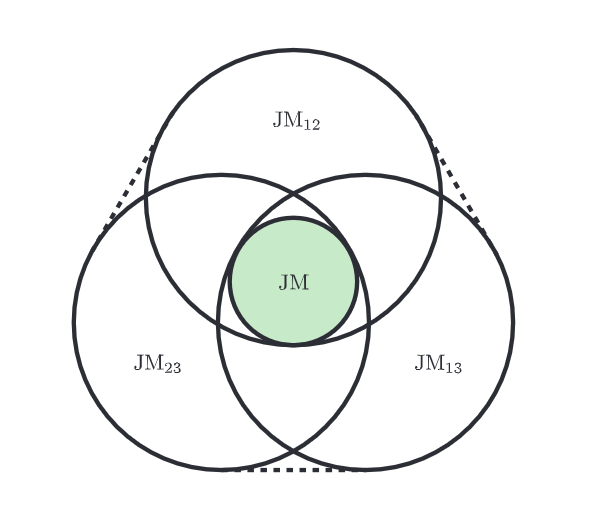
\includegraphics[width=0.38\textwidth]{convex-3-measurements}
  \caption{Convex-combination view of joint measurability for three
           noisy measurements, reproduced from Quintino
           \emph{et al.}~\cite{Quintino2019}: the family is jointly
           measurable iff it lies in the convex hull (shaded) of
           single-branch sub-families. $JM$ illustrates the set of
           fully jointly measurable families of MUBs, while $JM_{12}$,
           $JM_{13}$, $JM_{23}$ represent the sets of families in which
            the indicated pair is jointly measurable, with no constraint on the third measurement.}
  \label{fig:convex-3-measurements}
\end{wrapfigure}

Now that we have established certain robustness bounds for the joint measurability of $k$ MUBs, 
we can explore a more general notion of compatibility, which is the $k$-wise incompatibility of $k$ MUBs.
More specifically, we are interested in finding a probabilistic mixture of strategies, in each of which only one pair of the k measurements is jointly measured and the remaining k-2 are measured independently that would yield a valid and identically distributed measurement for each of the $k$ MUBs, and we want to find the noise-robustness threshold for this compatibility scenario.
This is a natural generalization of the full joint measurability scenario, and it is quite clear, and proved in the following, that this specific program will yield higher robustness thresholds.
\newline 
First, let us generalize the notion of genuine incompatibility from ~\cite{Quintino2019} to genuine k-wise incompatibility:
\newline
A set of
$k$ measurements is genuinely $k$-wise incompatible
when it cannot be written as a convex combination of strategies of $k-1$ 
measurements where 2 are jointly measured and the rest are measured individually. By this, we mean choosing a measurement strategy in which we probabilistically choose a pair of measurements
$i \neq j$ with $i, j \in \llbracket 1, k \rrbracket $ and perform a joint measurement for that pair while measuring the rest individually.
\newline
More formally, we have a probability matrix $P_{ij}$ with $i, j \in \llbracket 1, k \rrbracket $ and $i \neq j$, such that $\sum_{i < j} P_{ij} = 1$, and we have a set of parent POVMs $\{G^{(ij)}_{\lambda}\}$ for each pair of measurements $i \neq j$, such that the marginals of $G^{(ij)}_{\lambda}$ recover the noisy MUB measurements at settings $i$ and $j$.
\newline Geometrically (Figure~\ref{fig:convex-3-measurements}), the feasibility of this SDP amounts to asking whether the noisy family $\{M^{\eta}_{a|j}\}$ lies in the convex hull of the single-branch jointly-measurable families.
Figure ~\ref{fig:convex-3-measurements} illustrates why the noise-robustness threshold for full joint measurability is lower than the noise-robustness threshold for pairwise joint measurability: the set of fully jointly measurable families of MUBs (JM) is a strict subset of the convex hull of the pairwise jointly measurable families $(JM_{12}, JM_{13}, JM_{23})$.
\newline
The baseline program becomes: 
\newline
\begin{center}
\begin{align*}
&\text{find}      & & J_{a|x}^{(ij)},\ p_{ij},\ E_\lambda^{(ij)}\ \text{for all } i,j \in \llbracket 1,k \rrbracket,\ i<j \\
&\text{such that} & & E_\lambda^{(ij)} \geq 0,\quad p_{ij} \geq 0, \\
&                 & & M_{a|x} = \sum_{i<j} p_{ij} J_{a|x}^{(ij)}, \\
&                 & & J_{a|x}^{(ij)} \geq 0,\ \forall a,x;\ \sum_a J_{a|x}^{(ij)} = \mathds{1} ,\ \forall x, \\
&                 & & J_{a|x}^{(ij)} = \sum_\lambda D_\lambda(a|x)\, E_\lambda^{(ij)}\ \text{for } x \in \{i,j\}.
\end{align*}
\end{center}
where $D_\lambda(a|x)$ is the deterministic response function for the parent POVM $G^{(ij)}_{\lambda}$, and the constraints ensure that each $J_{a|x}^{(ij)}$ is a valid measurement strategy that recovers the noisy MUB measurements at settings $i$ and $j$ as marginals, and that the overall decomposition of $M_{a|x}$ into these pairwise strategies is valid.
\newline
Notice that we cannot yet use convex optimization to solve this program, since the constraints are \textbf{not linear} due to the product of \textbf{variables} $p_{ij}$ and $J_{a|x}^{(ij)}$ in the decomposition of $M_{a|x}$.
However, we can easily fix this by integrating the probability matrix $p$ into the Joint measurement term $J$:


\begin{center}
\begin{align*}
&\text{find}      & & J_{a|x}^{(ij)},\ p_{ij},\ E_\lambda^{(ij)}\ \text{for all } i,j \in \llbracket 1,k \rrbracket,\ i<j \\
&\text{such that} & & E_\lambda^{(ij)} \geq 0,\quad p_{ij} \geq 0, \\
&                 & & M_{a|x} = \sum_{i<j} J_{a|x}^{(ij)}, \\
&                 & & J_{a|x}^{(ij)} \geq 0,\ \forall a,x;\ \sum_a J_{a|x}^{(ij)} = p_{ij} \mathds{1} ,\ \forall x, \\
&                 & & J_{a|x}^{(ij)} = \sum_\lambda D_\lambda(a|x)\, E_\lambda^{(ij)}\ \text{for } x \in \{i,j\}.
   \refstepcounter{equation}\tag{\theequation}\label{eq:joint-decomp}
\end{align*}
\end{center}

In order to quantify the noise-robustness threshold $\eta^*$ for the $k$-wise compatibility scenario, we 
add the maximization constraint and model the following constraints:
\begin{center}
  \begin{equation}
    \begin{aligned}
\eta M_{a|x} + (1-\eta)\operatorname{Tr}(M_{a|x}) \frac{\mathds{1}}{d} &= J^k_{a|x}, \\
J^k_{a|x} &= \sum_{i<j} J_{a|x}^{(ij)}.
\end{aligned}
  \end{equation}
\end{center}

Since, $J_{a|x}^{(ij)} = \sum_\lambda D_\lambda(a|x)\, E_\lambda^{(ij)}$, $E_\lambda^{(ij)}$ is proportional to a POVM and $\sum_{i < j}E_\lambda^{(ij)} $ is a POVM,
we can further simplify the program as follows:
\begin{center}
\begin{align*}
&\text{maximize} & & \eta \in [0,1] \\
&\text{such that} & & E_\lambda^{(ij)} \geq 0, \sum_\lambda E_\lambda^{(ij)} = \frac{\mathds{1}}{d} \sum_\lambda Tr(E_\lambda^{(ij)}),\ \forall i,j \in \llbracket 1,k \rrbracket,\ i<j, \\
& & & \frac{1}{d} \sum_\lambda \sum_{i < j} Tr(E_\lambda^{(ij)}) = 1 \\ 
 & & & \eta M_{a|x} + (1-\eta) Tr(M_{a|x}) \frac{\mathds{1}}{d} \geq \sum_\lambda D_\lambda(a|x) \sum_{i \neq x} E_\lambda^{(ix)}\ \forall a,x.
\end{align*}
\end{center}

Where we extend $E$ such that $E_\lambda^{(ij)} = E_\lambda^{(ji)}$ for $i > j$.
\newline This state of the program is easy to solve by a convex optimization engine as well as to write as an SDP for general $k$, which has been done in the \texttt{robustness\_hypergraph} routine of Appendix~\ref{app:robustness-code} (Listing~\ref{lst:robustness-hypergraph}), which takes as input the compatibility hypergraph produced by \texttt{hypergraph\_pair(k)}, and builds the convex program above with CVXPY, delegating the actual optimization to a standard interior-point SDP solver such as CLARABEL, SCS, or MOSEK.

We then identify a natural lower bound $\eta^*$ for the noise-robustness threshold of this $(k-1)$-wise compatibility scenario, 
which is obtained by an equal probability mixture of all $\binom{k}{2}$ pairwise strategies, i.e. $p_{ij} = \frac{1}{\binom{k}{2}}$ for all $i < j$.
To compute $\eta^*$, we must first acknowledge the noise-robustness threshold for the pairwise compatibility of measurements $i$ and $j$, from 
Designolle et al.~\cite{Designolle2019}, which is a tight bound for the particular case of $k = 2$:
\begin{equation}
  \eta^{\star}(2, d) = \frac{2 + \sqrt{d}}{2(\sqrt{d} + 1)}.
  \label{eq:designolle-k2}
\end{equation}

Call a branch $(j,\ell)$ \textbf{active for setting $x$} if $x \in \{j,\ell\}$, and \textbf{inactive} otherwise. In an active branch, setting $x$ is presented at noise level $\eta^\star(2,d)$; in an inactive branch, at noise level $1$.
\newline Now, let us fix a measurement setting
$x$. By MUB symmetry, 
$x$ belongs to exactly $k-1$
 active branches and to $ \binom{k}{2} - (k-1) $ inactive ones. 
By the affineness lemma the mixture equals $M^{\eta_{\text{eff}}}_{a|x}$
with:


% Then, we can compute $\eta^*$ by using simple combinatorial principles.
% \newline Every measurement scenario appears with equal probability, hence, we divide by $\binom{k}{2}$, which is the number of scenarios,
%  and we sum over the particular noise robustness of the measurements in each case. Then, instead of summing over measurements, we study appearance of each MUB in all measurements then multiply by $k$ since they all appear the same way.
% \newline
% Each MUB appears in $\binom{k-1}{1}$, since it is jointly measured once with each of the other pairwise strategies, and each of these strategies has a noise-robustness threshold of $\eta^{\star}(2, d)$, 
% then, in the rest($\binom{k}{2} - \binom{k-1}{1}$) of the scenarios it is measured by itself with robustness $1$.
% \newline Therefore, the formula for $\eta^*$ is given by:
\begin{equation}
\begin{aligned}
\eta_{\text{eff}} &= \frac{1}{\binom{k}{2}} \left( \binom{k-1}{1} \eta^{\star}(2, d) + \left( \binom{k}{2} - \binom{k-1}{1} \right) \cdot 1 \right) 
\end{aligned} \end{equation}
Symmetry guarantees that the same number of active branches cover every setting $x$, hence the mixture reconstructs the noisy MUB family uniformly.
By simplifying, we get:
\begin{equation}
\begin{aligned}
\eta_{\text{eff}} &= \frac{2}{k(k-1)} ((k-1) \eta^*(2, d) + \frac{k(k-1)}{2} - (k - 1)) \\ 
&= \frac{1}{k} (2 \eta^*(2, d) + k - 2) \\
&= 1 + \frac{1}{k} (\frac{2 + \sqrt{d}}{\sqrt{d} + 1} - 2) \\
&= 1 - \frac{\sqrt{d}}{k(\sqrt{d} + 1)} \label{eq:lower-bound-k-wise}
\end{aligned}
\end{equation} 

In the results section, we will see that, for the cases we compute numerical values, this lower bound is certified by the SDP, which leads us to 
believe that the optimal strategy in the general case is to choose each pairwise strategy with equal probability.
Another thing to note about this lower bound (which holds for our computed values) is that it is \textbf{decreasing} in $d$, just like the noise-robustness threshold for Joint measurability,
however it is \textbf{increasing} in $k$, unlike the threshold for Joint Measurability.
\newline Let us develop on the latter conclusion in more detail: Adding a
measurement to the full-JM hypergraph enlarges the parent POVM by a
factor of $d$ and imposes one more marginal constraint, making the
joint POVM strictly harder to find. Adding a measurement to the
pairwise hypergraph, on the other hand, only adds new branches: the
decomposition gains $k$ more sub-strategies, each of which has to honour
the marginals of a single pair while leaving the remaining $k-2$
measurements as arbitrary POVMs. The ``responsibility'' of any fixed
measurement is consequently distributed across $k-1$ branches out of a
total of $\binom{k}{2}$, a vanishing fraction $2/k$ that becomes
negligible as $k$ grows. Quantitatively, this is exactly the
hierarchy of compatibility hypergraphs introduced by
Quintino~\emph{et al.}~\cite{Quintino2019}: finer hypergraphs (with
more, smaller hyperedges) yield monotonically larger noise tolerances,
and the all-pairs hypergraph -- being one of the finest non-trivial
structures -- yields one of the loosest possible relaxations of full
joint measurability.



\newpage
\section{Results}\label{sec:results}

\paragraph{Numerical setup.}
All SDPs were formulated with CVXPY and solved using
\textsc{Clarabel} for the small cases $d^k \le 100$ and \textsc{Scs} with
$\epsilon = 10^{-7}$, $\text{max\_iters} = 10^{5}$ for the larger ones,
on a standard laptop CPU. Cells with $d^k > 3000$ were omitted from
Table~\ref{tab:compat-prime} as the runtime exceeds 
minutes; Table~\ref{tab:pairwise-compat} has no such cap since the
pairwise SDP scales as $\mathcal{O}(k^3 d^2)$. Every closed-form entry
in Tables~\ref{tab:compat-prime} and~\ref{tab:pairwise-compat} agreed
with the analytical expression to within $10^{-4}$, and the solver
reported \texttt{optimal} (never \texttt{optimal\_inaccurate}) status
for all reported cells.

In this section, we present the numerical results obtained. In the first table, we reproduce the noise-robustness thresholds for the joint measurability of $k$ MUBs, while in the second 
table, we study the values obtained for the generalized $k$-wise incompatibility (for prime dimensions), that we obtained with our new generalized program.
Note that we are able to expand the second table much more than the first one, which at first could seem counterintuitive since the pairwise hypergraph is generating more constraints on the optimization problem.
\newline However, the parent POVM of a Joint measurement has $d^k$ outcomes, hence in the full joint measurability scenario, we are optimizing over $d^k$ positive semidefinite matrices
of size $d \times d$, a number that grows \emph{exponentially} with $k$.
In contrast, the pairwise hypergraph contains $\binom{k}{2}$ branches,
each of which carries a parent POVM with only $d^2$ outcomes plus
$(k-2)$ independent single-measurement POVMs; the total variable count
is therefore $\binom{k}{2}\bigl(d^2 + (k-2)\,d\bigr) = \mathcal{O}(k^3 d + k^2 d^2)$,
which grows only \emph{cubically} with $k$. The same gap shows up in
the marginal constraints, where the full-Jointly Measurable SDP sums $d^{k-1}$ matrices
per equality while the pairwise SDP sums only $d$ matrices per branch.
Concretely, for $(k=8,\, d=7)$ the full-Jointly Measurable SDP would require
$7^{8} \approx 5.76 \cdot 10^{6}$ matrix variables (intractable on any
desktop), while the pairwise SDP requires
$\binom{8}{2}(7^{2} + 6\cdot 7) = 2{,}548$ matrix variables which can
be solved in seconds, even on CPU. For this reason, we were able to 
populate table ~\ref{tab:pairwise-compat} up to $k = 11$ and $d = 9$ in less than 10 minutes, 
while having to omit even a few seemingly small entries from table ~\ref{tab:compat-prime}, such as $(k, d) = (5,5)$.


\begin{table}[h]
  \centering
  \caption{Numerical values for measurement compatibility:
           noise-robustness thresholds $\eta^{\star}(k, d)$ for the joint
           measurability of $k$ MUBs in prime dimension $d$. Closed-form
           entries are taken from \cite{Designolle2019} (or, for the
           complete set $k = d+1$, from its Theorem~1, which gives
           $\eta^{\star}(d+1, d) = 1/\sqrt{d+1}$); cells marked ``X''
           have been omitted due to computational complexity; the closed forms can be found in \cite{Designolle2019}. ``---'' marks
           cells with $k > d+1$, for which fewer than $k$ MUBs exist.}
  \label{tab:compat-prime}
  \renewcommand{\arraystretch}{1.4}
  \begin{tabular}{c|cccc}
    \hline
        & \multicolumn{4}{c}{$d$} \\
    \cline{2-5}
    $k$ & $2$ & $3$ & $5$ & $7$ \\
    \hline
    $2$ & $\tfrac{1}{\sqrt{2}}\!\approx\!0.7071$
        & $\tfrac{1+\sqrt{3}}{4}\!\approx\!0.6830$
        & $\tfrac{3+\sqrt{5}}{8}\!\approx\!0.6545$
        & $\tfrac{5+\sqrt{7}}{12}\!\approx\!0.6371$ \\
    $3$ & $\tfrac{1}{\sqrt{3}}\!\approx\!0.5774$
        & $\tfrac{\cos(\pi/18)}{\sqrt{3}}\!\approx\!0.5686$
        & $\tfrac{1+\sqrt{5}}{6}\!\approx\!0.5393$
        & $0.5101$ \\
    $4$ & ---
        & $\tfrac{1}{2}=0.5000$
        & 0.4615  &  0.4436 \\
    $5$ & ---
        & ---
        & $X$
        & $X$ \\
    $6$ & ---
        & ---
        & $\tfrac{1}{\sqrt{6}}\!\approx\!0.4082$
        & $X$ \\
    $7$ & ---
        & ---
        & ---
        & $X$ \\
    $8$ & ---
        & ---
        & ---
        & $\tfrac{1}{\sqrt{8}}\!\approx\!0.3536$ \\
    \hline
  \end{tabular}
\end{table}

\begin{table}[h]
  \centering
  \caption{Noise-robustness thresholds for the all-pairs compatibility hypergraph on $k$ MUBs in prime dimension $d$, computed 
  by the SDP of Section~5.3 with hypergraph \texttt{hypergraph\_pair(k)}. The 
  hyperedges are all $\binom{k}{2}$ pairs of settings; below the threshold the noisy MUB family admits a convex decomposition 
  into pairwise-jointly-measurable sub-experiments and is therefore not genuinely incompatible with respect to 
  this structure. All entries coincide with the closed form $\eta^\star = 1 - \sqrt{d}/(k(\sqrt{d}+1))$ derived in 
  Eq. ~\ref{eq:lower-bound-k-wise}, confirming optimality of the equal-weight pairwise mixture to solver precision. ``---'' marks cells with $k > d+1$.}
  \label{tab:pairwise-compat}
  \renewcommand{\arraystretch}{1.4}
  \begin{tabular}{c|ccccc}
    \hline
        & \multicolumn{5}{c}{$d$} \\
    \cline{2-6}
    $k$ & $2$ & $3$ & $5$ & $7$ & $11$ \\
    \hline
    2  &  0.7071  &  0.6830  &  0.6545  &  0.6371  &  0.6158   \\
    3  &  0.8047  &  0.7887  &  0.7697  &  0.7581  &  0.7439   \\
    4  &    ---     &  0.8415  &  0.8273  &  0.8186  &  0.8079   \\
    5  &    ---     &    ---     &  0.8618  &  0.8549  &  0.8463   \\
    6  &    ---     &    ---     &  0.8848  &  0.8791  &  0.8719   \\
    7  &    ---     &    ---     &    ---     &  0.8963  &  0.8902   \\
    8  &    ---     &    ---     &    ---     &  0.9093  &  0.9040   \\
    9  &    ---     &    ---     &    ---     &    ---     &  0.9146  \\
    \hline
  \end{tabular}
\end{table}

\FloatBarrier   % flush both Results tables before the next section starts
% \newpage

\section{Conclusion and Outlook}

In this work we reviewed the recent literature on the joint
measurability of quantum measurements and reproduced, by explicitly
formulating and solving the corresponding SDP, the known
noise-robustness thresholds for the joint measurability of $k$ MUBs in
prime dimension $d$. We then generalised this program to arbitrary
compatibility hypergraphs, exposing a single framework in which full
joint measurability is the trivial case. Using this
generalisation we computed new noise-robustness thresholds for the
all-pairs hypergraph and derived a closed-form analytical lower bound
that, in every case we checked numerically, is certified by the SDP to
solver precision.

\paragraph{Numerical contribution.}
Across $d \in \{2, 3, 5, 7, 11\}$ and all valid $k$, our SDP
reproduces every closed-form entry of Designolle
\emph{et al.}~\cite{Designolle2019} to within $10^{-4}$ (Table~\ref{tab:compat-prime})
and extends the table to the all-pairs hypergraph
(Table~\ref{tab:pairwise-compat}), with every entry matching the
analytical bound $\eta^{\star} = 1 - \sqrt{d}/[\,k(\sqrt{d}+1)\,]$
of \eqref{eq:lower-bound-k-wise}.

\paragraph{Qualitative findings.}
The most striking qualitative finding is that the noise-robustness
threshold of the pairwise hypergraph is \textbf{monotonically increasing}
in $k$, while the corresponding threshold for full joint measurability
is \textbf{monotonically decreasing} in $k$. The two thresholds therefore
diverge as $k$ grows: full joint measurability becomes harder, whereas
pairwise compatibility becomes easier, because each measurement's
``responsibility'' in a pairwise decomposition is distributed across
$k-1$ of the $\binom{k}{2}$ branches -- a vanishing fraction~$2/k$.
This is the quantitative illustration, on the MUB family, of the
hierarchy of compatibility hypergraphs introduced by
Quintino~\emph{et al.}~\cite{Quintino2019}, and it sharply illustrates
why genuine $k$-wise incompatibility is a strictly stronger notion than
pairwise incompatibility.

\paragraph{Going further.}
Three directions follow naturally from this work.
\begin{enumerate}
  \item[(i)] \emph{A tightness certificate.} Implementing the dual SDP
        would either prove tightness of \eqref{eq:lower-bound-k-wise}
        analytically -- by exhibiting a feasible dual witness whose
        objective matches $1 - \sqrt{d}/[\,k(\sqrt{d}+1)\,]$ -- or
        identify the regime where the equal-weight pairwise mixture is
        sub-optimal.
  \item[(ii)] \emph{Intermediate hypergraphs.} Between the two extremes
        we studied lies a rich lattice of compatibility hypergraphs --
        all triples, all $(k\!-\!2)$-subsets, asymmetric structures,
        and so on. Our framework already handles these without further
        modification; only their analytical behaviour remains
        unexplored.
  \item[(iii)] \emph{Composite dimensions.} The Wootters--Fields
        construction guarantees $d+1$ MUBs only for prime-power $d$;
        in $d = 6$ no fourth MUB has ever been found, and it is widely
        conjectured that none exists~\cite{Guhne2023}. Running the
        same hypergraph SDP for the three known MUBs in $d = 6$, and
        comparing the result to the prime-dimension pattern, would
        provide indirect evidence on this longstanding open question.
\end{enumerate}


\section*{Acknowledgements}
I am grateful to my advisors Marc-Olivier Renou and Lucas-Amadeus
Tendick for their guidance throughout this project, as well as to the
\textsc{PhIQuS} group at Inria Paris-Saclay for hosting me.

\newpage
\bibliographystyle{plain}
\bibliography{main}

\newpage
\appendix

\section{Appendix}
\label{sec:appendix}

\subsection{Hypergraph-parameterized robustness SDP}
\label{app:robustness-code}

The Python function below implements the white-noise robustness SDP
generalised to an arbitrary compatibility hypergraph~$C$, as discussed in
Section~\ref{sec:generalization-pairwise-jm}. It is built on top of CVXPY and delegates
variable creation, base constraints and inter-branch gluing to the
helper routines \texttt{\_build\_variables},
\texttt{\_base\_constraints} and \texttt{\_glue\_terms} (defined in the
accompanying source file \texttt{compatibility\_hypergraph.py}); it
returns the optimal $\eta^{\star}$ together with the solver's reported
status.

\begin{lstlisting}[style=python,
                   caption={\texttt{robustness\_hypergraph}: noise-robustness SDP for an arbitrary compatibility hypergraph.},
                   label=lst:robustness-hypergraph]
def robustness_hypergraph(M, hypergraph, *,
                          solver="CLARABEL", **solver_kwargs) -> tuple[float, str]:
    """
    Max eta such that the noisy version of M admits a decomposition.

    Returns (eta_star, solver_status).
    """
    m, n_a, d, _ = M.shape
    I = np.eye(d)
    hypergraph = [tuple(sorted(edge)) for edge in hypergraph]
    E, J_outside, p = _build_variables(M, hypergraph)
    cons = _base_constraints(M, hypergraph, E, J_outside, p)
    eta = cp.Variable()
    
    for x in range(m):
        for a in range(n_a):
            noisy = eta * M[x, a] + (1 - eta) * np.trace(M[x, a]) * I / d
            cons.append(sum(_glue_terms(x, a, hypergraph, E, J_outside)) == noisy)
    prob = cp.Problem(cp.Maximize(eta), cons)
    prob.solve(solver=solver, **solver_kwargs)
    return float(eta.value), prob.status
\end{lstlisting}

\begin{lstlisting}[style=python,
                   caption={\texttt{\_glue\_terms}: helper function that builds the list of contributions from each branch to $M_{x|a}$.},
                   label=lst:glue-terms]
def _glue_terms(x, a, hypergraph, E, J_outside):
    """For (x, a), build the list of contributions from each branch to M[x, a]."""
    terms = []
    for i, edge in enumerate(hypergraph):
        if x in edge:
            terms.append(_marginal_E(E[i], edge, x, a))
        else:
            terms.append(J_outside[i][x][a])
    return terms
\end{lstlisting}

\subsection{The two hypergraphs we provide in the above function to generate our results}
\label{app:hypergraph-helpers}

The two helper functions below construct the compatibility hypergraphs
corresponding to the two extreme cases of interest. Both are intended to
be passed as the \texttt{hypergraph} argument of
\texttt{robustness\_hypergraph} (Listing~\ref{lst:robustness-hypergraph})
together with a measurement family of $k$ POVMs.

\begin{lstlisting}[style=python,
                   caption={Helpers for the two extremal compatibility hypergraphs.},
                   label=lst:hypergraph-helpers]
def hypergraph_compatible(k):
    """Compatibility hypergraph for the given number of POVMs."""
    hypergraph = [tuple(range(k))]
    return hypergraph

def hypergraph_pair(k):
    """Compatibility hypergraph with all pairs of POVMs."""
    hypergraph = [tuple(edge) for edge in itertools.combinations(range(k), 2)]
    return hypergraph
\end{lstlisting}

\paragraph{Full joint measurability:
\texttt{hypergraph\_compatible(k)}.}
This returns the trivial hypergraph
$C = \{\,(0, 1, \dots, k-1)\,\}$ consisting of a single hyperedge that
contains \emph{all} $k$ measurement settings. Plugged into
\texttt{robustness\_hypergraph}, the resulting SDP collapses to a single
branch in which all $k$ noisy measurements are required to share a
common parent POVM~$\{G_\lambda\}$ with
$\lambda \in [n_a]^k$. The optimisation thus reduces exactly to the
standard $k$-wise joint-measurability robustness program
\eqref{eq:sdp-robustness-kmub}, whose optimal value reproduces the
classical noise-robustness thresholds tabulated in Table~I of
\cite{Designolle2019}. This is the \emph{tightest} constraint
available---no other hypergraph yields a smaller~$\eta^{\star}$.

\paragraph{All pairs:
\texttt{hypergraph\_pair(k)}.}
This returns the hypergraph
$C = \{\,(j, \ell) : 0 \le j < \ell \le k-1\,\}$ consisting of all
$\binom{k}{2}$ unordered pairs. Each branch~$i$ corresponds to one
pair~$(j, \ell)$ and asks for a joint POVM that reproduces only the
marginals of measurements~$j$ and~$\ell$, while the remaining $k - 2$
measurements are represented by arbitrary, independent POVMs in that
branch. The SDP then searches for the maximal~$\eta$ such that the
noisy family $\{M^{\eta}_{a|x}\}$ can be written as a convex (i.e.\
probabilistic) mixture of these pairwise-joint sub-experiments,
\begin{equation*}
  M^{\eta}_{a|x} \;=\; \sum_{(j,\ell)} p_{(j,\ell)}\,
                          M^{(x), (j,\ell)}_{a},
  \qquad p_{(j,\ell)} \ge 0,\;\; \sum_{(j,\ell)} p_{(j,\ell)} = 1,
\end{equation*}
with each branch satisfying the joint-measurability constraint only on
its own pair. Operationally, the experimenter selects a pair at random
with probability~$p_{(j,\ell)}$ and runs the corresponding pairwise
joint measurement; this exactly reproduces the observed statistics
whenever the SDP is feasible. The resulting~$\eta^{\star}$ is the
white-noise threshold below which the family is \emph{not genuinely
$k$-wise incompatible} in the sense of~\cite{Quintino2019}: pairwise
joint measurability is enough to simulate the data. Since this
hypergraph imposes strictly weaker constraints than full joint
measurability, its threshold is monotonically larger than the one given
by \texttt{hypergraph\_compatible(k)} (cf.\
Section~\ref{sec:sdp-2qubit}).


\end{document}